% Configurazione
\documentclass[12pt, a4paper]{report}

\usepackage{graphicx}
\usepackage[table,xcdraw]{xcolor}
%\usepackage{xcolor}
\usepackage{float}
\usepackage{titlesec}
\usepackage[utf8]{inputenc}
\usepackage{hyperref}
\usepackage{float}
\usepackage{caption}
\usepackage{fancyhdr}
\usepackage{geometry}
\usepackage{longtable}
\usepackage[italian]{babel}
\usepackage{longtable}
\usepackage{array}
\newcolumntype{L}[1]{>{\raggedright\arraybackslash}p{#1}}
\newcolumntype{C}[1]{>{\centering\arraybackslash}p{#1}}
\newcolumntype{R}[1]{>{\raggedleft\arraybackslash}p{#1}}

\hypersetup{
    colorlinks=true,
    linkcolor=black,
    urlcolor=blue,
}

\geometry{
  top=30mm,
  bottom=30mm,
  left=30mm,
  right=30mm,
}

\pagestyle{fancy}
\lhead{}
\lfoot{Analisi dei requisiti}
\cfoot{}
\rfoot{\thepage}
\renewcommand{\headrulewidth}{0.4pt}
\renewcommand{\footrulewidth}{0.4pt}
\setlength{\headheight}{16pt}

\fancypagestyle{firstpage}{%
  \renewcommand{\headrulewidth}{0pt}%
  \renewcommand{\footrulewidth}{0pt}%
  \lfoot{}
  \rfoot{}
}

\graphicspath{ {immagini/} }
\definecolor{RossoUnipd}{HTML}{B5121B}
\titleformat{\chapter}{\normalfont\huge}{\thechapter.}{20pt}{\huge\textbf}
\newcommand{\todo}[1]{\textcolor{red}{TODO: #1}}

% Variabili
\newcommand{\titolo}{Analisi dei Requisiti}
%\newcommand{\req}[1]{%
  %\begin{tabular}{@{}c@{}}\strut#1\strut\end{tabular}%
%}



% Struttura
\begin{document}
  \thispagestyle{firstpage}
  \begin{minipage}[]{0.3\textwidth}
  
\includegraphics[width=0.8\textwidth]{logo_uni}
\end{minipage}
\begin{minipage}[]{0.6\textwidth}
  \textcolor{RossoUnipd}{
    \textbf{Università degli Studi di Padova} \\
    Laurea: Informatica \\
    Corso: Ingegneria del Software \\
    Anno Accademico: 2021/2022
  }
\end{minipage}

\bigskip

\begin{minipage}[]{0.3\textwidth}
  
\includegraphics[width=0.8\textwidth]{logo_merl}
\end{minipage}
\begin{minipage}[]{0.6\textwidth}
  Gruppo: MERL \\
  Email: \texttt{merlunipd@gmail.com}
\end{minipage}

\bigskip
\bigskip
\bigskip

  \begin{center}
  \Huge\textbf{Verbale Riunione}
\end{center}

\begin{center}
  \LARGE\textbf{01 Aprile 2022}
\end{center}

\bigskip
\bigskip
\bigskip

  \newpage
  \begin{center}
  \huge{Registro delle Modifiche}
\end{center}
\renewcommand\arraystretch{1,5}
{\centering
\begin{longtable}{|C{1.8cm}|C{2.1cm}|C{2cm}|C{2.4cm}|L{4.4cm}|}
  \hline
  \rowcolor[HTML]{036400}
  \textcolor[HTML]{FFFFFF}{\textbf{Versione}} & \textcolor[HTML]{FFFFFF}{\textbf{Data}} & \textcolor[HTML]{FFFFFF}{\textbf{Autore}}  & \textcolor[HTML]{FFFFFF}{\textbf{Verificatore}} & \textcolor[HTML]{FFFFFF}{\textbf{Modifica}}    \\ \hline
  \rowcolor[HTML]{EFEFEF}
  v2.0.0        & 04/05/2022    & Mattia Zanellato   &  -  & Approvazione \\ \hline
  \rowcolor[HTML]{C0C0C0}
  v1.0.15       & 04/05/2022    & Mattia Zanellato   &  Marco Mazzucato  & Aggiunta sottosezione "Decimo Periodo" in "Consuntivo" \\ \hline
  \rowcolor[HTML]{EFEFEF}
  v1.0.14       & 27/04/2022    & Emanuele Pase   &   Marco Mazzucato & Aggiunta sottosezione "Decimo Periodo" in "Preventivo" \\ \hline
  \rowcolor[HTML]{C0C0C0}
  v1.0.13       & 26/04/2022    & Riccardo Contin   &  Emanuele Pase  & Aggiunta sottosezione "Nono Periodo" in "Consuntivo" \\ \hline
  \rowcolor[HTML]{EFEFEF}
  v1.0.12       & 21/04/2022    & Riccardo Contin   &  Marco Mazzucato   & Aggiunta sottosezione "Nono Periodo" in "Pianificazione" e in "Preventivo" \\ \hline
  \rowcolor[HTML]{C0C0C0}
  v1.0.11       & 19/04/2022    & Emanuele Pase   &  Marco Mazzucato   & Aggiunta sottosezione "Ottavo Periodo" in "Consuntivo" \\ \hline
  \rowcolor[HTML]{EFEFEF}
  v1.0.10       & 15/04/2022    & Emanuele Pase   &  Marco Mazzucato   & Aggiunta sottosezione "Ottavo Periodo" in "Preventivo" \\ \hline
  \rowcolor[HTML]{C0C0C0}
  v1.0.9        & 13/04/2022    & Marco Mazzucato   &  Riccardo Contin   & Aggiunta sottosezione "Settimo Periodo" in "Consuntivo" \\ \hline
  \rowcolor[HTML]{EFEFEF}
  v1.0.8        & 06/04/2022    & Lorenzo Onelia   &  Riccardo Contin    & Aggiunta sottosezione "Sesto Periodo" in "Consuntivo" \\ \hline
  \rowcolor[HTML]{C0C0C0}
  v1.0.7        & 06/04/2022    & Marco Mazzucato   &   Lorenzo Onelia   & Aggiunta sottosezione "Settimo Periodo" in "Preventivo" \\ \hline
  \rowcolor[HTML]{EFEFEF}
  v1.0.6        & 06/04/2022    & Marco Mazzucato   &  Lorenzo Onelia    & Aggiunta sottosezione "Settimo Periodo" in "Pianificazione" \\ \hline
  \rowcolor[HTML]{C0C0C0}
  v1.0.7        & 31/03/2022    & Lorenzo Onelia   &  Marco Mazzucato    & Aggiunta sottosezione "Sesto Periodo" in "Preventivo" \\ \hline
  \rowcolor[HTML]{EFEFEF}
  v1.0.6        & 31/03/2022    & Lorenzo Onelia   &   Marco Mazzucato   & Aggiunta sottosezione "Sesto Periodo" in "Pianificazione" \\ \hline
  \rowcolor[HTML]{C0C0C0}
  v1.0.5        & 28/03/2022    & Marco Mamprin   &  Marco Mazzucato    & Aggiunta sottosezione "Quinto Periodo" in "Consuntivo" \\ \hline
  \rowcolor[HTML]{EFEFEF}
  v1.0.4        & 27/03/2022    & Marko Vukovic   &  Riccardo Contin    & Aggiunta sottosezione "Semaforo Rosso RTB" in "Consuntivo" \\ \hline
  \rowcolor[HTML]{C0C0C0}
  v1.0.3        & 24/03/2022    & Lorenzo Onelia  & Emanuele Pase    & Fix minori                  \\ \hline
  \rowcolor[HTML]{EFEFEF}
  v1.0.2        & 24/03/2022    & Marco Mamprin   &  Lorenzo Onelia    & Aggiunta sottosezione "Quinto Periodo" in "Preventivo" \\ \hline
  \rowcolor[HTML]{C0C0C0}
  v1.0.1        & 24/03/2022    & Marco Mamprin   &  Lorenzo Onelia    & Aggiunta sottosezione "Quinto Periodo" in "Pianificazione" \\ \hline
  \rowcolor[HTML]{EFEFEF}
  v1.0.0        & 08/03/2022    & Marko Vukovic   &  -                 & Approvazione \\ \hline
  \rowcolor[HTML]{C0C0C0}
  v0.0.17       & 04/03/2022    & Lorenzo Onelia  & Mattia Zanellato     & Aggiunta Lista di distribuzione                  \\ \hline
  \rowcolor[HTML]{EFEFEF}
  v0.0.16       & 24/02/2022     & Riccardo Contin  & Lorenzo Onelia                                & Fix finali \\ \hline
  \rowcolor[HTML]{C0C0C0}
  v0.0.15       & 23/02/2022    & Riccardo Contin   & Lorenzo Onelia                  & Pianificazione futura \\ \hline
  \rowcolor[HTML]{EFEFEF}
  v0.0.14       & 23/02/2022    & Mattia Zanellato  & Marko Vukovic                   & Aggiunta sottosezione "Quarto Periodo" in "Consuntivo" \\ \hline
  \rowcolor[HTML]{C0C0C0}
  v0.0.13       & 17/02/2022    & Riccardo Contin   & Mattia Zanellato                & Modifiche capitolo "Consuntivo" \\ \hline
  \rowcolor[HTML]{EFEFEF}
  v0.0.12       & 16/02/2022    & Mattia Zanellato  & Lorenzo Onelia                  & Aggiunto capitolo "Organigramma" \\ \hline
  \rowcolor[HTML]{C0C0C0}
  v0.0.11       & 11/02/2022    & Mattia Zanellato  & Riccardo Contin                 & Aggiunto capitolo "Mitigazione dei Rischi" \\ \hline
  \rowcolor[HTML]{EFEFEF}
  v0.0.10       & 10/02/2022    & Mattia Zanellato  & Lorenzo Onelia                  & Aggiunto capitolo "Modello di Sviluppo" \\ \hline
  \rowcolor[HTML]{C0C0C0}
  v0.0.9        & 08/02/2022    & Mattia Zanellato  & Lorenzo Onelia                  & Aggiunta sottosezione "Quarto Periodo" in "Preventivo" \\ \hline
  \rowcolor[HTML]{EFEFEF}
  v0.0.8        & 06/02/2022    & Mattia Zanellato  & Lorenzo Onelia                  & Aggiunta sottosezione "Terzo Periodo" in "Consuntivo" \\ \hline
  \rowcolor[HTML]{C0C0C0}
  v0.0.7        & 04/02/2022    & Emanuele Pase     & Marco Mamprin                   & Modifiche capitolo "Pianificazione" \\ \hline
  \rowcolor[HTML]{EFEFEF}
  v0.0.6        & 13/01/2022    & Emanuele Pase     & Marco Mamprin Riccardo Contin   & Aggiunta sottosezione "Secondo Periodo" in "Consuntivo" e sottosezione "Terzo Periodo" in "Preventivo" \\ \hline
  \rowcolor[HTML]{C0C0C0}
  v0.0.5        & 07/01/2022    & Riccardo Contin   & Lorenzo Onelia                  & Aggiunto capitolo "Introduzione" \\ \hline
  \rowcolor[HTML]{EFEFEF}
  v0.0.4        & 28/12/2021    & Riccardo Contin   & Lorenzo Onelia                  & Aggiunta sottosezione "Primo Periodo" in "Consuntivo" e sottosezione "Secondo Periodo" in "Preventivo" \\ \hline
  \rowcolor[HTML]{C0C0C0}
  v0.0.3        & 15/12/2021    & Riccardo Contin   & Marco Mamprin                   & Aggiunta sottosezione "Primo Periodo" in "Preventivo" \\ \hline
  \rowcolor[HTML]{EFEFEF}
  v0.0.2        & 11/12/2021    & Riccardo Contin   & Marco Mamprin                   & Aggiunto capitolo "Analisi dei rischi" \\ \hline
  \rowcolor[HTML]{C0C0C0}
  v0.0.1        & 08/12/2021    & Riccardo Contin   & Marco Mamprin                   & Aggiunto capitolo "Pianificazione" \\ \hline
  \rowcolor[HTML]{EFEFEF}
  v0.0.0        & 07/12/2021    & Riccardo Contin   & Marco Mamprin                   & Creata prima struttura del documento \\ \hline
\end{longtable}}

\renewcommand\arraystretch{1}

  \tableofcontents
  \listoftables
  \listoffigures
  % Capitoli
  \chapter{Introduzione}
\section{Premessa}

Il \textit{Piano di Qualifica} è un documento su cui si prevede di lavorare per l'intera durata del progetto. Molti contenuti di questo documento sono di natura instabile, come alcune metriche che non sono applicabili nella fase iniziale e che solo con il loro utilizzo pratico si può valutarne l'effettiva utilità. Anche i processi selezionati possono essere soggetti a cambiamenti, dato che possono rivelarsi insufficienti o inadeguati agli scopi del progetto e al modo di lavorare del gruppo.
Per tutte queste ragioni il documento è prodotto in maniera incrementale e suoi comntenuti iniziali sono da considerarsi incompleti.

\section{Scopo del documento}
Il \textit{Piano di Qualifica} è un documento che:
\begin{itemize}
    \item Specifica gli obiettivi
    quantitativi di qualità di prodotto e di processo;
    \item Espone le
    metodologie di controllo e le misurazioni di queste qualità tramite
    opportune metriche;
    \item Definisce quanti e quali test eseguire per verificare il corretto funzionamento
    e la qualità dei processi e del prodotto;
    \item Applica questi test e ne documenta l'esito;
    \item Crea un cruscotto di supporto che fornisce
    una visione dello stato corrente degli obiettivi.
\end{itemize}

\section{Scopo del prodotto}
Il capitolato proposto dall'azienda \textit{Zucchetti S.p.A} ha come obiettivo
quello di creare un'applicazione di visualizzazione di dati con numerose dimensioni
che permettono di rintracciare eventuali anomalie attraverso l'occhio umano. Lo
scopo del prodotto è quindi quello di fornire all'utente diversi tipi di
visualizzazione di dati in modo da rendere più veloce ed efficacie l'individuazione
di anomalie.

\section{Glossario}
Per evitare ambiguità relative alle terminoligie utilizzate è stato creato il \textit{Glossario v1.0.0} nel quale sono riportati tutti i termini importanti o con un significato particolare.
\section{Riferimenti}
\subsection{Riferimenti normativi}
\begin{itemize}
  \item \textit{Norme di Progetto v1.0.0}
\end{itemize}
\subsection{Riferimenti informativi}
\begin{itemize}
  \item \textbf{Capitolato d'appalto C5 - Login Warrior}
          \url{https://www.math.unipd.it/~tullio/IS-1/2021/Progetto/C5.pdf}
  \item \textbf{Qualità di processo}
          \url{https://www.math.unipd.it/~tullio/IS-1/2021/Dispense/T13.pdf}
  \item \textbf{Qualità di prodotto}
          \url{https://www.math.unipd.it/~tullio/IS-1/2021/Dispense/T12.pdf}
  \item \textbf{Verifica e validazione}
          \url{https://www.math.unipd.it/~tullio/IS-1/2021/Dispense/T14.pdf}
          \url{https://www.math.unipd.it/~tullio/IS-1/2021/Dispense/T15.pdf}
          \url{https://www.math.unipd.it/~tullio/IS-1/2021/Dispense/T16.pdf}
  \item \textbf{Ciclo di Deming}
          \url{https://it.wikipedia.org/wiki/Ciclo_di_Deming}
  \item \textbf{Indice di Gulpease}
          \url{https://it.wikipedia.org/wiki/Indice_Gulpease}
\end{itemize}

  \chapter{Descrizione}

\section{Obiettivi del Prodotto}
Il prodotto deve essere in grado di visualizzare dati a molte dimensioni sotto forma di diversi grafici, per supportare la fase di analisi attraverso l'utilizzo di tecnologie web.

\section{Funzioni del Prodotto}
L'applicazione si occupa di analizzare uno o più set di dati e di restituire dei grafici che risultano essere più comprensibili e significativi.
Con l'utilizzo di grafici appositamente creati e in base a filtri selezionati dall'utente che permettono varie visualizzazioni, è possibile estrapolare informazioni che in un primo momento potevano essere poco chiare o nascoste.
È possibile anche salvare le informazioni in un file scaricabile in formato JSON$_G$, in modo da poter successivamente ripristinare la sessione nel punto in cui era stata interrotta.

  \chapter{Casi d'Uso}
\section*{Inizializzazione sistema}

\begin{figure}[ht]
  \centering
  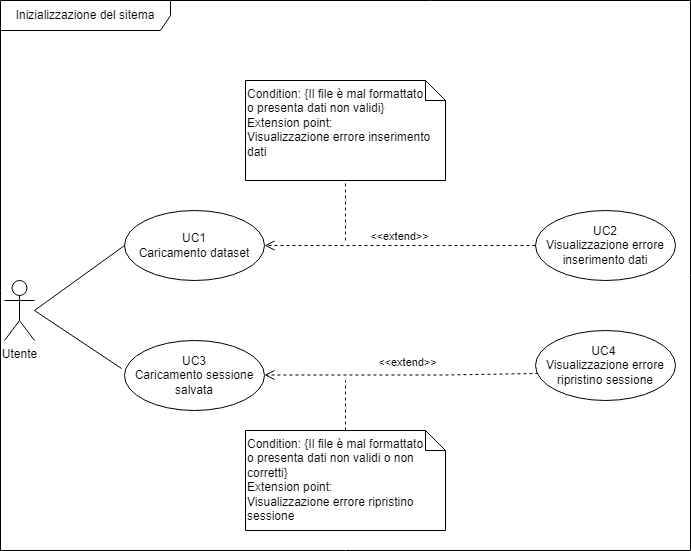
\includegraphics[width=\textwidth]{Iniz_sistema}
  \caption{Inizializzazione del sistema}
\end{figure}
\section{UC1 - Caricamento dataset}
\begin{itemize}
  \item \textbf{Descrizione:} l'utente vuole analizzare un nuovo dataset non presente nel sistema;
  \item \textbf{Attore primario:} utente;
  \item \textbf{Precondizioni:} il sistema è raggiungibile e funzionante. L’utente ha a disposizione un dataset in formato CSV;
  \item \textbf{Postcondizioni:} i dati presenti nel file vengono caricati nel sistema.
  \item \textbf{Scenario principale:}
  \begin{enumerate}
    \item L'utente accede al sistema;
    \item L'utente sceglie un file in formato CSV presente in locale e lo carica nel sistema;
    \item L'utente è pronto ad analizzare i dati.
  \end{enumerate}
  \item \textbf{Estensioni:} nel caso in cui il file sia in un formato non valido o i dati non siano validi:
    \begin{enumerate}
      \item Il caricamento non va a buon fine;
      \item Viene visualizzato un errore esplicativo [UC2].
    \end{enumerate}
\end{itemize}

\section{UC2 - Visualizzazione errore inserimento dati}
\begin{itemize}
  \item \textbf{Descrizione}: l'utente carica un file mal formattato o che presenta dati non validi, quindi visualizza un messaggio di errore esplicativo;
  \item \textbf{Attore Primario:} utente;
  \item \textbf{Precondizioni:} l’utente carica un file CSV contenente i dati da analizzare mal formattato o che presenta dati non validi;
  \item \textbf{Postcondizioni:} l'utente visualizza un messaggio di errore e i dati non vengono caricati;
  \item \textbf{Scenario Principale:}
  \begin{enumerate}
    \item L'utente visualizza un messaggio di errore esplicativo.
  \end{enumerate}
\end{itemize}

\section{UC3 - Caricamento sessione salvata}
\begin{itemize}
  \item \textbf{Descrizione:} l'utente vuole riprendere ad analizzare da dove si era interrotto o ha la necessità di visualizzare una sessione precedente;
  \item \textbf{Attore Primario:} utente;
  \item \textbf{Precondizioni:} l'utente che avvia l'applicativo ha salvato almeno una sessione di lavoro precedente;
  \item \textbf{Postcondizioni:} i dati di una sessione precedentemente salvata vengono ricaricati nel sistema;
  \item \textbf{Scenario Principale:}
  \begin{enumerate}
    \item L'utente accede al sistema;
    \item L'utente sceglie la sessione da caricare selezionando il file JSON desiderato tra quelli disponibili,
    cioè tra le sessioni salvate in precedenza;
    \item L'utente riprende da dove aveva salvato.
  \end{enumerate}
  \item \textbf{Estensioni:} nel caso in cui il file JSON selezionato non sia leggibile per qualche possibile errore di salvataggio:
    \begin{enumerate}
      \item Fallisce il caricamento della sessione precedente;
      \item Viene visualizzato un errore esplicativo [UC4].
    \end{enumerate}
\end{itemize}

\section{UC4 - Visualizzazione errore ripristino sessione}
\begin{itemize}
  \item \textbf{Descrizione}: l'utente carica un file mal formattato o che presenta dati non corretti, quindi visualizza un messaggio di errore esplicativo;
  \item \textbf{Attore Primario:} utente;
  \item \textbf{Precondizioni:} l’utente carica un file JSON contenente i dati da analizzare mal formattato o che presenta dati non validi o non corretti;
  \item \textbf{Postcondizioni:} l'utente visualizza un messaggio di errore e i dati non vengono caricati;
  \item \textbf{Scenario Principale:}
  \begin{enumerate}
    \item L'utente visualizza un messaggio di errore esplicativo.
  \end{enumerate}
\end{itemize}

\section{UC5 - Selezione tipo di grafico}
\begin{figure}[H]
 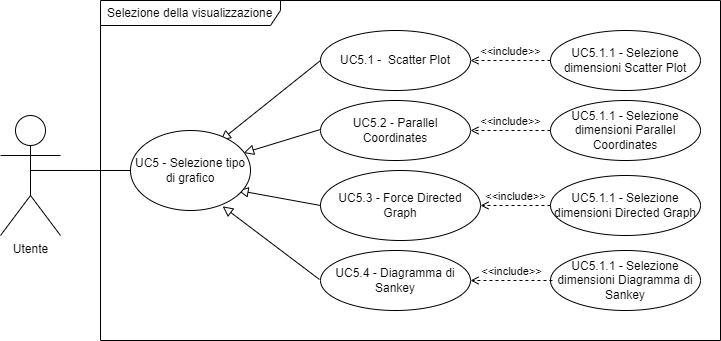
\includegraphics[width=\textwidth]{uc5.png}
 \caption{UC5 - Selezione tipo di grafico}
\end{figure}

 \begin{itemize}
     \item \textbf{Descrizione:} l'utente visualizza varie tipologie di grafico e ne sceglie una;
     \item \textbf{Attore primario:} utente;
     \item \textbf{Precondizioni:} il sistema è stato inizializzato [UC1];
     \item \textbf{Postcondizioni:} viene visualizzato il grafico desiderato;
     \item \textbf{Scenario principale:}
     \begin{enumerate}
       \item L'utente sceglie la visualizzazione desiderata tra quelle disponibili;
     \end{enumerate}
     \item \textbf{Generalizzazioni:} l'utente può selezionare una tra le possibili opzioni:
     \begin{enumerate}
         \item \textit{Scatter Plot} [UC5.1];
         \item \textit{Parallel Coordinates} [UC5.2];
         \item \textit{Force-Directed Graph} [UC5.3];
         \item \textit{Sankey Diagram} [UC5.4].
     \end{enumerate}
 \end{itemize}

\subsection{UC5.1 - Selezione Scatter Plot}
\begin{itemize}
    \item \textbf{Descrizione:} l'utente decide che visualizzazione di \textit{Scatter Plot} vuole vedere;
    \item \textbf{Attore primario:} utente;
    \item \textbf{Precondizioni:} il sistema è stato inizializzato [UC1];
    \item \textbf{Postcondizioni:} viene visualizzato il grafico \textit{Scatter Plot} selezionato;
    \item \textbf{Scenario principale:}
    \begin{enumerate}
      \item L'utente sceglie la visualizzazione desiderata tra quelle disponibili, decidendo tra varie visualizzazioni dello stesso grafico.
    \end{enumerate}
\end{itemize}

\subsection{UC5.2 - Selezione Parallel Coordinates}
\begin{itemize}
    \item \textbf{Descrizione:} l'utente decide che visualizzazione di \textit{Parallel Coordinates} vuole vedere;
    \item \textbf{Attore primario:} utente;
    \item \textbf{Precondizioni:} il sistema è stato inizializzato [UC1];
    \item \textbf{Postcondizioni:} viene visualizzato il grafico \textit{Parallel Coordinates} selezionato;
    \item \textbf{Scenario principale:}
    \begin{enumerate}
    \item L'utente sceglie la visualizzazione desiderata tra quelle disponibili, decidendo tra varie visualizzazioni dello stesso grafico.
    \end{enumerate}
\end{itemize}

\subsection{UC5.3 - Selezione Force-Directed Graph}
\begin{itemize}
    \item \textbf{Descrizione:} l'utente decide che visualizzazione di \textit{Force-Directed Graph} vuole vedere;
    \item \textbf{Attore primario:} utente;
    \item \textbf{Precondizioni:} il sistema è stato inizializzato [UC1];
    \item \textbf{Postcondizioni:} viene visualizzato il grafico \textit{Force-Directed Graph} selezionato;
    \item \textbf{Scenario principale:}
    \begin{enumerate}
      \item L'utente sceglie la visualizzazione desiderata tra quelle disponibili, decidendo tra varie visualizzazioni dello stesso grafico.
    \end{enumerate}
\end{itemize}

\subsection{UC5.4 - Selezione Sankey Diagram}
\begin{itemize}
    \item \textbf{Descrizione:} l'utente decide che visualizzazione di \textit{Sankey Diagram} vuole vedere;
    \item \textbf{Attore primario:} utente;
    \item \textbf{Precondizioni:} il sistema è stato inizializzato [UC1];
    \item \textbf{Postcondizioni:} viene visualizzato il grafico \textit{Sankey Diagram} selezionato;
    \item \textbf{Scenario principale:}
    \begin{enumerate}
      \item L'utente sceglie la visualizzazione desiderata tra quelle disponibili, decidendo tra varie visualizzazioni dello stesso grafico.
    \end{enumerate}
\end{itemize}


\section{UC6 - Filtri sui dati}
\begin{figure}[H]
  \centering
  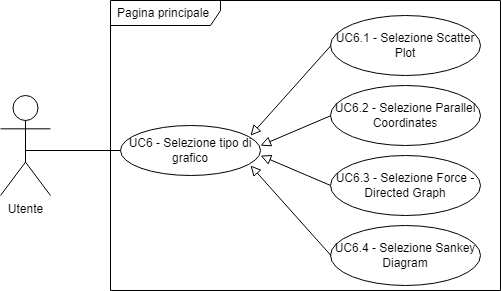
\includegraphics[width=\textwidth]{uc6.png}
  \caption{UC6 - Filtri sui dati}
\end{figure}

\begin{itemize}
  \item \textbf{Descrizione}: l'utente ha la possibilità di modificare la visualizzazione attraverso l'applicazione di filtri sui dati;
  \item \textbf{Attore primario}: utente;
  \item \textbf{Precondizioni}: l'utente ha selezionato la tipologia di grafico [UC5] e l'applicativo lo ha generato;
  \item \textbf{Postcondizioni}: i filtri applicati consentono di mostrare la nuova visualizzazione dei dati sul grafico;
  \item \textbf{Scenario principale}:
    \begin{enumerate}
      \item L'utente può impostare i seguenti filtri tramite una sezione dedicata:
        \begin{itemize}
          \item ID [UC6.1];
          \item IP [UC6.2];
          \item Utente [UC6.3];
          \item Evento [UC6.4];
          \item Data [UC6.5];
          \item Applicazione [UC6.6].
        \end{itemize}
      \item Il grafico mostra solo i dati con le caratteristiche corrispondenti alla scelta dei filtri.
    \end{enumerate}
\end{itemize}

\subsection{UC6.1 - Filtraggio per ID}
\begin{itemize}
  \item \textbf{Descrizione}: l'utente ha la possibilità di filtrare i dati in base ad un determinato ID;
  \item \textbf{Attore primario}: utente;
  \item \textbf{Precondizioni}: l'utente ha selezionato la tipologia di grafico [UC5] e l'applicativo lo ha generato;
  \item \textbf{Postcondizioni}: i dati visualizzati sono filtrati in base ad un determinato ID;
  \item \textbf{Scenario principale}:
    \begin{enumerate}
      \item L'utente inserisce l'ID desiderato;
      \item Il grafico mostra solo i dati con l'ID corrispondente.
    \end{enumerate}
\end{itemize}

\subsection{UC6.2 - Filtraggio per IP}
\begin{itemize}
  \item \textbf{Descrizione}: l'utente ha la possibilità di filtrare i dati in base ad un determinato IP;
  \item \textbf{Attore primario}: utente;
  \item \textbf{Precondizioni}: l'utente ha selezionato la tipologia di grafico [UC5] e l'applicativo lo ha generato;
  \item \textbf{Postcondizioni}: i dati visualizzati sono filtrati in base ad un determinato IP;
  \item \textbf{Scenario principale}:
    \begin{enumerate}
      \item L'utente inserisce l'IP desiderato;
      \item Il grafico mostra solo i dati con l'IP corrispondente.
    \end{enumerate}
\end{itemize}

\subsection{UC6.3 - Filtraggio per utente}
\begin{itemize}
  \item \textbf{Descrizione}: l'utente ha la possibilità di filtrare i dati in base ad un determinato utente;
  \item \textbf{Attore primario}: utente;
  \item \textbf{Precondizioni}: l'utente ha selezionato la tipologia di grafico [UC5] e l'applicativo lo ha generato;
  \item \textbf{Postcondizioni}: i dati visualizzati sono filtrati in base ad un determinato utente;
  \item \textbf{Scenario principale}:
    \begin{enumerate}
      \item L'utente inserisce il numero dell'utente desiderato;
      \item Il grafico mostra solo i dati con il numero dell'utente corrispondente.
    \end{enumerate}
\end{itemize}

\subsection{UC6.4 - Filtraggio per evento}
\begin{itemize}
  \item \textbf{Descrizione}: l'utente ha la possibilità di filtrare i dati in base ad un determinato tipo di evento;
  \item \textbf{Attore primario}: utente;
  \item \textbf{Precondizioni}: l'utente ha selezionato la tipologia di grafico [UC5] e l'applicativo lo ha generato;
  \item \textbf{Postcondizioni}: i dati visualizzati sono filtrati in base ad un determinato tipo di evento;
  \item \textbf{Scenario principale}:
    \begin{enumerate}
      \item L'utente inserisce il tipo di evento desiderato;
      \item Il grafico mostra solo i dati con il tipo di evento corrispondente.
    \end{enumerate}
\end{itemize}

\subsection{UC6.5 - Filtraggio per data}
\begin{itemize}
  \item \textbf{Descrizione}: l'utente ha la possibilità di filtrare i dati in base alla data;
  \item \textbf{Attore primario}: utente;
  \item \textbf{Precondizioni}: l'utente ha selezionato la tipologia di grafico [UC5] e l'applicativo lo ha generato;
  \item \textbf{Postcondizioni}: i dati visualizzati sono filtrati in base alla data;
  \item \textbf{Scenario principale}:
    \begin{enumerate}
      \item L'utente inserisce il periodo temporale desiderato;
      \item Il grafico mostra solo i dati interni al periodo temporale corrispondente.
    \end{enumerate}
\end{itemize}

\subsection{UC6.6 - Filtraggio per applicazione}
\begin{itemize}
  \item \textbf{Descrizione}: l'utente ha la possibilità di filtrare i dati in base ad una determinata applicazione;
  \item \textbf{Attore primario}: utente;
  \item \textbf{Precondizioni}: l'utente ha selezionato la tipologia di grafico [UC5] e l'applicativo lo ha generato;
  \item \textbf{Postcondizioni}: i dati visualizzati sono filtrati in base ad una determinata applicazione;
  \item \textbf{Scenario principale}:
    \begin{enumerate}
      \item L'utente inserisce l'applicazione desiderata;
      \item Il grafico mostra solo i dati relativi all'applicazione corrispondente.
    \end{enumerate}
\end{itemize}


\section{UC7 - Accesso al manuale utente}
\begin{itemize}
  \item \textbf{Descrizione}: l'utente che ha un dubbio o vuole più informazioni sull'utilizzo dell'applicazione, deve avere accesso rapido al manuale utente;
  \item \textbf{Attore primario}: utente;
  \item \textbf{Precondizioni}: nessuna, l'opzione di accesso ai manuali deve essere sempre disponibile all'utente;
  \item \textbf{Postcondizioni}: viene visualizzato il manuale utente;
  \item \textbf{Scenario principale}:
  \begin{enumerate}
    \item L'utente seleziona il manuale utente;
    \item Viene visualizzato il manuale utente.
  \end{enumerate}
\end{itemize}

\section{UC8 - Salvataggio sessione}
\begin{itemize}
  \item \textbf{Descrizione:} l'utente salva la sessione di lavoro;
  \item \textbf{Attore primario:} utente;
  \item \textbf{Precondizioni:} l'utente ha svolto una sessione di lavoro sull'applicazione, in particolare potrebbe aver scelto un grafico specifico e modificato i parametri personalizzando la visualizzazione;
  \item \textbf{Postcondizioni:} l'utente possiede un file JSON in grado di recuperare grafico e parametri impostati durante la sessione di lavoro;
  \item \textbf{Scenario principale:}
  \begin{enumerate}
    \item L'utente sta lavorando sull'applicazione;
    \item L'utente seleziona la funzionalità ``Salvataggio sessione'';
    \item L'utente salva la sessione corrente.
  \end{enumerate}
\end{itemize}

  \chapter{Requisiti}

\renewcommand\arraystretch{1,5}

\section{Introduzione}
Il gruppo \textit{MERL} dopo un'attenta analisi ha individuato i seguenti requisiti che il prodotto finale andrà a soddisfare. Questi sono organizzati in forma tabellare e la loro struttura segue le regole definite nel documento \textit{Norme di Progetto}.

\section{Requisiti Funzionali}

\begin{center}
  \centering
  \begin{longtable}{|L{2cm}|C{5,5cm}|C{3cm}|C{2cm}|}
    \hline
    \rowcolor[HTML]{036400}
    \textcolor[HTML]{FFFFFF}{\textbf{Codice}} & \textcolor[HTML]{FFFFFF}{\textbf{Descrizione}} & \textcolor[HTML]{FFFFFF}{\textbf{Classificazione}} & \textcolor[HTML]{FFFFFF}{\textbf{Fonti}}
    \\ \hline
    \rowcolor[HTML]{EFEFEF}
    RF.1.1 & L'utente deve poter caricare i dati tramite un nuovo dataset & Obbligatorio & Capitolato - UC1 \\ \hline
    \rowcolor[HTML]{C0C0C0}
    RF.1.2 & Visualizzazione messaggio di errore in caso di problemi durante il caricamento dati & Obbligatorio & UC2 \\ \hline
    \rowcolor[HTML]{EFEFEF}
    RF.2.3 & L'utente deve poter caricare una sessione precedentemente salvata & Desiderabile & UC3 \\ \hline
    \rowcolor[HTML]{C0C0C0}
    RF.1.4 & Visualizzazione messaggio di errore in caso di problemi durante il caricamento della sessione & Obbligatorio & UC4 \\ \hline
    \rowcolor[HTML]{EFEFEF}
    RF.1.5 & L'utente deve poter selezionare il grafico da visualizzare & Obbligatorio & Capitolato - UC5 \\ \hline
    \rowcolor[HTML]{C0C0C0}
    RF.1.5.1 & L'utente deve poter selezionare il grafico \textit{Scatter Plot} & Obbligatorio & Capitolato - UC5.1 \\ \hline
    \rowcolor[HTML]{EFEFEF}
    RF.1.5.2 & L'utente deve poter selezionare il grafico \textit{Parallel Coordinates} & Obbligatorio & Capitolato - UC5.2 \\ \hline
    \rowcolor[HTML]{C0C0C0}
    RF.1.5.3 & L'utente deve poter selezionare il grafico \textit{Force-Direct Graph} & Obbligatorio & Capitolato - UC5.3 \\ \hline
    \rowcolor[HTML]{EFEFEF}
    RF.1.5.4 & L'utente deve poter selezionare il grafico \textit{Sankey Diagram} & Obbligatorio & Capitolato - UC5.4 \\ \hline
    \rowcolor[HTML]{C0C0C0}
    RF.1.? & L'utente deve poter personalizzare la visualizzazione scelta & Obbligatorio & UC? \\ \hline
    \rowcolor[HTML]{EFEFEF}
    RF.1.?.1.1 & L'utente deve poter modificare la visualizzazione dei punti & Obbligatorio & UC?.1 \\ \hline
    \rowcolor[HTML]{C0C0C0}
    RF.1.?.1.2 & L'utente deve poter scegliere i colori & Obbligatorio & UC?.1 \\ \hline
    \rowcolor[HTML]{EFEFEF}
    RF.2.?.3.1 & L'utente deve poter scegliere la funzione di forza & Desiderabile & UC?.3 \\ \hline
    \rowcolor[HTML]{C0C0C0}
    RF.1.?.3.2 & L'utente deve poter scegliere l'intensità delle forze di tensione e repulsione & Obbligatorio & UC?.3 \\ \hline
    \rowcolor[HTML]{EFEFEF}
    RF.1.?.3.3 & L'utente deve poter scegliere gli stili per la visualizzazione del grafico & Obbligatorio & UC?.3 \\ \hline
    \rowcolor[HTML]{C0C0C0}
    RF.2.?.4.1 & L'utente deve poter scegliere la colorazione dei link & Obbligatorio & UC?.4 \\ \hline
    \rowcolor[HTML]{EFEFEF}
    RF.1.?.4.2 & L'utente deve poter impostare l'opacità dei link & Obbligatorio & UC?.4 \\ \hline
    \rowcolor[HTML]{C0C0C0}
    RF.2.?.4.3 & L'utente deve poter scegliere l'allinamento dei link & Desiderabile & UC?.4 \\ \hline
    \rowcolor[HTML]{EFEFEF}
    RF.1.7 & Visualizzazione messaggio di errore in caso di filtri scelti in modo scorretto & Obbligatorio & UC7 \\ \hline
    \rowcolor[HTML]{C0C0C0}
    RF.2.8 & L'utente deve poter accedere al manuale utente & Desiderabile & UC8 \\ \hline
    \rowcolor[HTML]{EFEFEF}
    RF.2.9 & L'utente deve poter salvare la sessione in corso & Desiderabile & UC9 \\ \hline

    \caption{Tabella dei requisiti funzionali}
  \end{longtable}
\end{center}

\section{Requisiti di Qualità}
\begin{center}
  \centering
  \begin{longtable}{|L{1,5cm}|C{5,5cm}|C{3cm}|C{2cm}|}
    \hline
    \rowcolor[HTML]{036400}
    \textcolor[HTML]{FFFFFF}{\textbf{Codice}} & \textcolor[HTML]{FFFFFF}{\textbf{Descrizione}} & \textcolor[HTML]{FFFFFF}{\textbf{Classificazione}} & \textcolor[HTML]{FFFFFF}{\textbf{Fonti}}
    \\ \hline
    \rowcolor[HTML]{EFEFEF}
    RQ.1.1 & Deve essere fornito un manuale utente per l'utilizzo & Obbligatorio & Capitolato \\ \hline
    \rowcolor[HTML]{C0C0C0}
    RQ.1.2 & Il prodotto deve essere open source & Obbligatorio & Capitolato \\ \hline
    \rowcolor[HTML]{EFEFEF}
    RQ.1.3 & Il codice sorgente deve essere presente su una repository in \textit{GitHub} o in altri repository pubblici & Obbligatorio & Capitolato \\ \hline
    \rowcolor[HTML]{C0C0C0}
    RQ.1.4 & Il prodotto deve essere sviluppato seguendo le \textit{Norme di Progetto} & Obbligatorio & \textit{Norme di Progetto} \\ \hline

    \caption{Tabella dei requisiti di qualità}
  \end{longtable}
\end{center}

\section{Requisiti di Vincolo}
\begin{center}
  \centering
  \begin{longtable}{|L{1,5cm}|C{5,5cm}|C{3cm}|C{2cm}|}
    \hline
    \rowcolor[HTML]{036400}
    \textcolor[HTML]{FFFFFF}{\textbf{Codice}} & \textcolor[HTML]{FFFFFF}{\textbf{Descrizione}} & \textcolor[HTML]{FFFFFF}{\textbf{Classificazione}} & \textcolor[HTML]{FFFFFF}{\textbf{Fonti}}
    \\ \hline
    \rowcolor[HTML]{EFEFEF}
    RV.1.1 & L'interfaccia grafica deve essere sviluppata in \textit{HTML}/\textit{CSS} & Obbligatorio & Capitolato \\ \hline
    \rowcolor[HTML]{C0C0C0}
    RV.1.2 & I grafici devono essere realizzati tramite l'utilizzo di \textit{Javascript} & Obbligatorio & Capitolato \\ \hline
    \rowcolor[HTML]{EFEFEF}
    RV.1.3 & Il prodotto finale deve essere in grado di analizzare file \textit{CSV} & Obbligatorio & Capitolato \\ \hline
    \rowcolor[HTML]{C0C0C0}
    RV.3.4 & Deve essere utilizzata la libreria \textit{D3.js} & Opzionale & Capitolato \\ \hline
    \rowcolor[HTML]{EFEFEF}
    RV.1.5 & Il prodotto finale è supportato dai seguenti browser: \textit{Chrome 61}, \textit{Edge 16}, \textit{Firefox 60}, \textit{Opera 48}, \textit{Safari 10.1} & Obbligatorio & \textit{Javascript Modules} \\ \hline


    \caption{Tabella dei requisiti di vincolo}
  \end{longtable}
\end{center}

\section{Requisiti Prestazionali}
Il gruppo \textit{MERL} non ha individuato alcun requisito prestazionale durante l'analisi del capitolato e delle richieste del proponente.


\section{Tracciamento}

\subsection{Fonte - Requisiti}
\begin{center}
  \centering
  \begin{longtable}{|C{6cm}|C{6cm}|}
    \hline
    \rowcolor[HTML]{036400}
    \textcolor[HTML]{FFFFFF}{\textbf{Fonte}} & \textcolor[HTML]{FFFFFF}{\textbf{Requisiti}} \\ \hline
    \rowcolor[HTML]{EFEFEF}
    Capitolato & RF.1.1 - RF.1.5 - RF.1.5.1 - RF.1.5.2 - RF.1.5.3 - RF.1.5.4 - RQ.1.1 - RQ.1.2 - RQ.1.3 - RV.1.1 - RV.1.2 - RV.1.3 - RV.3.4 \\ \hline
    \rowcolor[HTML]{C0C0C0}
    UC1 & RF.1.1 \\ \hline
    \rowcolor[HTML]{EFEFEF}
    UC2 & RF.1.2 \\ \hline
    \rowcolor[HTML]{C0C0C0}
    UC3 & RF.2.3 \\ \hline
    \rowcolor[HTML]{EFEFEF}
    UC4 & RF.1.4 \\ \hline
    \rowcolor[HTML]{C0C0C0}
    UC5 & RF.1.5 \\ \hline
    \rowcolor[HTML]{EFEFEF}
    UC5.1 & RF.1.5.1 \\ \hline
    \rowcolor[HTML]{C0C0C0}
    UC5.2 & RF.1.5.2 \\ \hline
    \rowcolor[HTML]{EFEFEF}
    UC5.3 & RF.1.5.3 \\ \hline
    \rowcolor[HTML]{C0C0C0}
    UC5.4 & RF.1.5.4 \\ \hline
    \rowcolor[HTML]{EFEFEF}
    UC? & RF.1.? \\ \hline
    \rowcolor[HTML]{C0C0C0}
    UC?.1 & RF.1.?.1.1 RF.1.?.1.2 \\ \hline
    \rowcolor[HTML]{EFEFEF}
    UC?.3 & RF.2.?.3.1 RF.1.?.3.2 RF.1.?.3.3  \\ \hline
    \rowcolor[HTML]{C0C0C0}
    UC?.4 & RF.1.?.4.1 RF.1.?.4.2 RF.2.?.4.3  \\ \hline
    \rowcolor[HTML]{EFEFEF}
    UC7 & RF.1.7 \\ \hline
    \rowcolor[HTML]{C0C0C0}
    UC8 & RF.2.8 \\ \hline
    \rowcolor[HTML]{EFEFEF}
    UC9 & RF.2.9 \\ \hline
    \rowcolor[HTML]{C0C0C0}
    \textit{Norme di Progetto} & RQ.1.4 \\ \hline
    \rowcolor[HTML]{EFEFEF}
    R.V.1.2 & RV.1.5 \\ \hline

    \caption{Tabella di tracciamento fonte-requisiti}
  \end{longtable}
\end{center}

\subsection{Requisito - Fonti}
\begin{center}
  \centering
  \begin{longtable}{|C{6cm}|C{6cm}|}
    \hline
    \rowcolor[HTML]{036400}
    \textcolor[HTML]{FFFFFF}{\textbf{Requisito}} & \textcolor[HTML]{FFFFFF}{\textbf{Fonti}} \\ \hline
    \rowcolor[HTML]{EFEFEF}
    RF.1.1 & Capitolato - UC1 \\ \hline
    \rowcolor[HTML]{C0C0C0}
    RF.1.2 & UC2 \\ \hline
    \rowcolor[HTML]{EFEFEF}
    RF.2.3 & UC3 \\ \hline
    \rowcolor[HTML]{C0C0C0}
    RF.1.4 & UC4 \\ \hline
    \rowcolor[HTML]{EFEFEF}
    RF.1.5 & Capitolato - UC5 \\ \hline
    \rowcolor[HTML]{C0C0C0}
    RF.1.5.1 & Capitolato - UC5.1 \\ \hline
    \rowcolor[HTML]{EFEFEF}
    RF.1.5.2 & Capitolato - UC5.2 \\ \hline
    \rowcolor[HTML]{C0C0C0}
    RF.1.5.3 & Capitolato - UC5.3 \\ \hline
    \rowcolor[HTML]{EFEFEF}
    RF.1.5.4 & Capitolato - UC5.4 \\ \hline
    \rowcolor[HTML]{C0C0C0}
    RF.1.? & UC? \\ \hline
    \rowcolor[HTML]{EFEFEF}
    RF.1.?.1.1 & UC?.1 \\ \hline
    \rowcolor[HTML]{C0C0C0}
    RF.1.?.1.2 & UC?.1 \\ \hline
    \rowcolor[HTML]{EFEFEF}
    RF.2.?.3.1 & UC?.3 \\ \hline
    \rowcolor[HTML]{C0C0C0}
    RF.1.?.3.2 & UC?.3 \\ \hline
    \rowcolor[HTML]{EFEFEF}
    RF.1.?.3.3 & UC?.3 \\ \hline
    \rowcolor[HTML]{C0C0C0}
    RF.1.?.4.1 & UC?.4 \\ \hline
    \rowcolor[HTML]{EFEFEF}
    RF.1.?.4.2 & UC?.4 \\ \hline
    \rowcolor[HTML]{C0C0C0}
    RF.2.?.4.3 & UC?.4 \\ \hline
    \rowcolor[HTML]{EFEFEF}
    RF.1.7 & UC7 \\ \hline
    \rowcolor[HTML]{C0C0C0}
    RF.2.8 & UC9 \\ \hline
    \rowcolor[HTML]{EFEFEF}
    RF.2.9 & UC10 \\ \hline
    \rowcolor[HTML]{C0C0C0}
    RQ.1.1 & Capitolato \\ \hline
    \rowcolor[HTML]{EFEFEF}
    RQ.1.2 & Capitolato \\ \hline
    \rowcolor[HTML]{C0C0C0}
    RQ.1.3 & Capitolato \\ \hline
    \rowcolor[HTML]{EFEFEF}
    RQ.1.4 & \textit{Norme di Progetto} \\ \hline
    \rowcolor[HTML]{C0C0C0}
    RV.1.1 & Capitolato \\ \hline
    \rowcolor[HTML]{EFEFEF}
    RV.1.2 & Capitolato \\ \hline
    \rowcolor[HTML]{C0C0C0}
    RV.1.3 & Capitolato \\ \hline
    \rowcolor[HTML]{EFEFEF}
    RV.3.4 & Capitolato \\ \hline
    \rowcolor[HTML]{C0C0C0}
    RV.1.5 & RV.1.2 \\ \hline

    \caption{Tabella di tracciamento requisito-fonti}
  \end{longtable}
\end{center}


\section{Riepilogo}

\begin{center}
  \centering
  \begin{longtable}{|c|c|c|c|c|}
    \hline
    \rowcolor[HTML]{036400}
    {\color[HTML]{FFFFFF} \textbf{Tipologia}} & {\color[HTML]{FFFFFF} \textbf{Obbligatorio}} & {\color[HTML]{FFFFFF} \textbf{Desiderabile}} & {\color[HTML]{FFFFFF} \textbf{Opzionale}}  & {\color[HTML]{FFFFFF} \textbf{Totale}} \\ \hline
    \rowcolor[HTML]{EFEFEF}
    Funzionale & 16 & 5 & 0 & 21 \\ \hline
    \rowcolor[HTML]{C0C0C0}
    Di Qualità & 4 & 0 & 0 & 4 \\ \hline
    \rowcolor[HTML]{EFEFEF}
    Di Vincolo & 4 & 0 & 1 & 5 \\ \hline
    \rowcolor[HTML]{C0C0C0}
    Prestazionale & 0 & 0 & 0 & 0 \\ \hline

    \caption{Tabella del riepilogo totale}
  \end{longtable}
\end{center}

\end{document}
